\documentclass[a4paper,10pt]{article}
\usepackage{fullpage}
\usepackage[british]{babel}
\usepackage[T1]{fontenc}
\usepackage{amsmath}
\usepackage{amssymb}
\usepackage[T1]{fontenc}
\usepackage{natbib}
\usepackage[utf8]{inputenc}
%\usepackage{amsthm} \newtheorem{theorem}{Theorem}
\usepackage{color}
\usepackage{float}
\usepackage{authblk}
\usepackage{todonotes}
\usepackage{algorithmicx}
\usepackage{algpseudocode}% http://ctan.org/pkg/algorithmicx

\usepackage{caption}
\DeclareCaptionFont{white}{\color{white}}
\DeclareCaptionFormat{listing}{\colorbox{gray}{\parbox{\textwidth}{#1#2#3}}}
\captionsetup[lstlisting]{format=listing,labelfont=white,textfont=white}

\usepackage{alltt}
\usepackage{listings}
\usepackage{algorithm}
%\usepackage{algorithmicx}
\usepackage{subfig}
\lstset{% parameters for all code listings
language=Python,
frame=single,
basicstyle=\small, % nothing smaller than \footnotesize, please
tabsize=2,
numbers=left,
% framexleftmargin=2em, % extend frame to include line numbers
%xrightmargin=2em, % extra space to fit 79 characters
breaklines=true,
breakatwhitespace=true,
prebreak={/},
captionpos=b,
columns=fullflexible,
escapeinside={\#*}{\^^M}
}



\usepackage{tikz}
\usetikzlibrary{arrows}
\usetikzlibrary{automata,positioning}

\newcommand{\abpsender}[1][]{

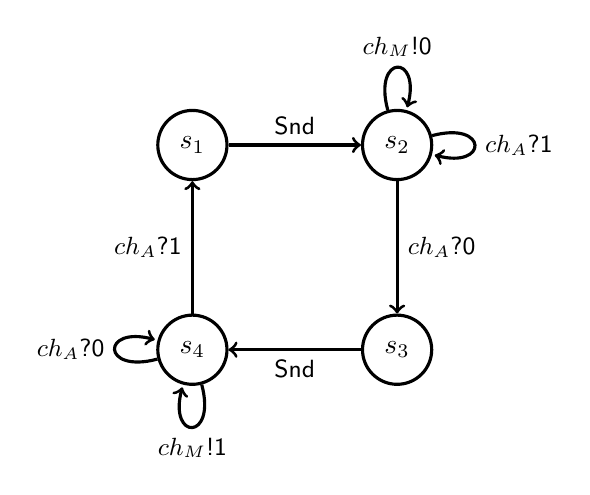
\begin{tikzpicture} [->,auto,node distance=2.6cm,line width=0.4mm]
  \node[state] (1) {$s_1$};
  \node[state] (2) [right of=1] {$s_2$};
  \node[state] (3) [below of=2] {$s_3$};
  \node[state] (4) [left of=3] {$s_4$};

  \path[every node/.style={font=\sffamily\small}]
    (1) edge node [above] {Snd} (2)
    (2) edge node [right] {$ch_A$?0} (3)
        edge [loop right] node {$ch_A$?1} (2)
        edge [loop above] node {$ch_M$!0} (2)
    (3) edge node [below] {Snd} (4)
    (4) edge node [left] {$ch_A$?1} (1)
        edge [loop left] node {$ch_A$?0} (4)
        edge [loop below] node {$ch_M$!1} (4);
\end{tikzpicture}
}

\newcommand{\abpreceiver}[1][]{
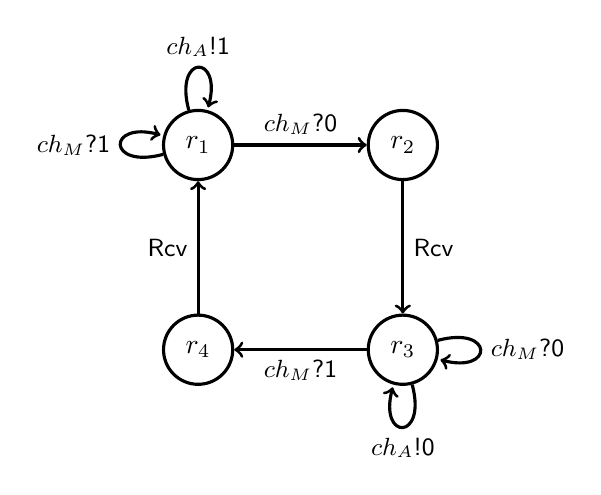
\begin{tikzpicture} [->,auto,node distance=2.6cm,line width=0.4mm]

  \node[state] (1) {$r_1$};
  \node[state] (2) [right of=1] {$r_2$};
  \node[state] (3) [below of=2] {$r_3$};
  \node[state] (4) [left of=3] {$r_4$};

  \path[every node/.style={font=\sffamily\small}]
    (1) edge node [above] {$ch_M$?0} (2)
        edge [loop left] node {$ch_M$?1} (1)
        edge [loop above] node {$ch_A$!1} (1)
    (2) edge node [right] {Rcv} (3)
    (3) edge node [below] {$ch_M$?1} (4)
        edge [loop right] node {$ch_M$?0} (3)
        edge [loop below] node {$ch_A$!0} (3)
    (4) edge node [left] {Rcv} (1);

\end{tikzpicture}
}

\newcommand{\abpobserver}[1][]{
\begin{tikzpicture} [->,auto,node distance=2.6cm,line width=0.4mm]

%\begin{tikzpicture}[->,>=stealth',shorten >=1pt,auto,node distance=3cm,
%  thick,main node/.style={circle,fill=blue!20,draw,font=\sffamily\Large\bfseries}]

  \node[state] (1) {$o_1$};
  \node[state,accepting] (3) [right of=1] {$o_2$};
  \node[state] (2) [right of=2] {$o_3$};

  \path[every node/.style={font=\sffamily\small}]
    (1) edge [bend left] node [above] {Snd} (2)
        edge node [above] {Rcv} (3)
    (2) edge [bend left] node [below] {Rcv} (1)
        edge node [above] {Snd} (3);
\end{tikzpicture}
}

% Alter some LaTeX defaults for better treatment of figures:
    % See p.105 of "TeX Unbound" for suggested values.
    % See pp. 199-200 of Lamport's "LaTeX" book for details.
    % General parameters, for ALL pages:
    \renewcommand{\topfraction}{0.9}	% max fraction of floats at top
    \renewcommand{\bottomfraction}{0.8}	% max fraction of floats at bottom
    % Parameters for TEXT pages (not float pages):
    \setcounter{topnumber}{2}
    \setcounter{bottomnumber}{2}
    \setcounter{totalnumber}{4} % 2 may work better
    \setcounter{dbltopnumber}{2} % for 2-column pages
    \renewcommand{\dbltopfraction}{0.9}	% fit big float above 2-col. text
    \renewcommand{\textfraction}{0.07}	% allow minimal text w. figs
    % Parameters for FLOAT pages (not text pages):
    \renewcommand{\floatpagefraction}{0.7}	% require fuller float pages
% N.B.: floatpagefraction MUST be less than topfraction !!
    \renewcommand{\dblfloatpagefraction}{0.7}	% require fuller float pages

% remember to use [htp] or [htpb] for placement


\usepackage{fancyvrb}
%\DefineVerbatimEnvironment{code}{Verbatim}{fontsize=\small
%\DefineVerbatimEnvironment{example}{Verbatim}{fontsize=\small}

\usepackage{url}
\urldef{\mailsa}\path|josh0151@student.uu.se |
\urldef{\mailsb}\path|bjfo5755@student.uu.se |
\newcommand{\keywords}[1]{\par\addvspace\baselineskip
\noindent\keywordname\enspace\ignorespaces#1}


\usepackage{tikz} \usetikzlibrary{trees}
\usepackage{hyperref} % should always be the last package

% useful colours (use sparingly!):
\newcommand{\blue}[1]{{\color{blue}#1}}
\newcommand{\green}[1]{{\color{green}#1}}
\newcommand{\red}[1]{{\color{red}#1}}

% useful wrappers for algorithmic/Python notation:
\newcommand{\length}[1]{\text{len}(#1)}
\newcommand{\twodots}{\mathinner{\ldotp\ldotp}} % taken from clrscode3e.sty
\newcommand{\Oh}[1]{\mathcal{O}\left(#1\right)}

% useful (wrappers for) math symbols:
\newcommand{\Cardinality}[1]{\left\lvert#1\right\rvert}
%\newcommand{\Cardinality}[1]{\##1}
\newcommand{\Ceiling}[1]{\left\lceil#1\right\rceil}
\newcommand{\Floor}[1]{\left\lfloor#1\right\rfloor}
\newcommand{\Iff}{\Leftrightarrow}
\newcommand{\Implies}{\Rightarrow}
\newcommand{\Intersect}{\cap}
\newcommand{\Sequence}[1]{\left[#1\right]}
\newcommand{\Set}[1]{\left\{#1\right\}}
\newcommand{\SetComp}[2]{\Set{#1\SuchThat#2}}
\newcommand{\SuchThat}{\mid}
\newcommand{\Tuple}[1]{\langle#1\rangle}
\newcommand{\Union}{\cup}
\newcommand{\conf}[1]{\langle#1\rangle}
\newcommand{\subword}{\sqsubseteq}
\newcommand{\e}[1]{\emph{#1}}
\usetikzlibrary{positioning,shapes,shadows,arrows}

\usepackage{url}


\usepackage{booktabs,array}
\def\Midrule{\midrule[\heavyrulewidth]}
\newcount\rowc

\makeatletter
\def\ttabular{%
\hbox\bgroup
\let\\\cr
\valign\bgroup
\global\rowc\@ne
\hbox to 7em{\strut \hfill##\hfill}%
&&%
\global\advance\rowc\@ne
\hbox to 7em{\strut\hfill##\hfill}%
\cr}
\def\endttabular{%
\crcr\egroup\egroup}


\usepackage{amsthm}
\theoremstyle{plain}
\newtheorem{theorem}{Theorem}
\newtheorem{corollary}{Corollary}[theorem]
\newtheorem{lemma}[theorem]{Lemma}



%Specific for this document


\title{\textbf{Algorithmic Analysis of Channel machines\\ Using Small Models}}

\author{Jonathan Sharyari}
\textwidth 5.5in 
\oddsidemargin 0.5in 


\begin{document}

\maketitle


abstract
\tableofcontents
\section{Proposal}
\subsection{Channel system}
A channel system L is a tuple $\langle$S,$s_0$,A,C,M,$\delta$$\rangle$, where
\begin{itemize}
\item[]
S is a finite set of control states,
\item[]
$s_0$ is an initial control state,
\item[]
A is a finite set of actions,
\item[]
C is a finite set of channels,
\item[]
M is a finite set of messages,
\item[]
$\delta$ is a finite set of transitions, each of which is a triple of the form $\rangle$s1,op,s2$\langle$, where s1 and s2 are control states, and op is a label of one of the forms

\begin{itemize}
\item
c!m, where c $\in$ C and m $\in$ M,
\item
c?m, where c $\in$ C and m $\in$ M,
\end{itemize}
\end{itemize}

\subsection{Channel transition system}

A channel system induces a transition system TS = (K, $\rightarrow$) where K=$(SC)^*$ and $\rightarrow$ $\subseteq$ K$\times$K is the transition relation.

Using $s_k$[i] to denote the state of the ith process and $c_k$[i] to denote the state of the ith channel of a configuration k=($s_k$, $c_k$), the transition relation $\rightarrow$ contains relations k $\rightarrow$ k' with

\begin{itemize}
  \item
    $s_k[i] \longrightarrow s_k'[i]$ for some i, with $\longrightarrow \in A$, and the states of all processes j$\neq$i and all channels remain unchanged by the transition.
  \item
    $c_k[i] \longrightarrow c_k'[i]$ for some i, with $\longrightarrow \in \delta$, and all other channels j$\neq$i and the states of all processes remain unchanged by the transition.
\end{itemize}

\subsection{Subwords and views}

Using $c_k[i]$ be a channel in a transition system k containing the word w=$w_1...w_l$ of length l, then the subword relation $\sqsubseteq$ is a relation (as described elsewere). Then a view v of a configuration k=($s_k,c_k$) (denoted v $\sqsubseteq$ k, with the symbol overloaded) is a tuple ($s_k, c_k'$) such that $c_k'$ $\sqsubseteq$ $c_k$.

\subsection{View abstraction}
The abstraction function $\alpha_p: K\rightarrow 2^{K_p}$ maps a configuration k into the set $\alpha_k(k) = \{v\in C_k | v\sqsubseteq K\}$. 

The concretization function $\gamma_k: 2^{K_p} \rightarrow 2^K$ inputs a set of views V $\subseteq$ $K_p$, and returns the set of configurations that can be reconstructed from the views in V, in other words, $\gamma_k(V) = \{k \in K | \alpha_p(k) \subseteq V$\}

The abstract post-image of a set of view V $\in$ $C_p$ is defined as $Apost_p$(V) = $\alpha_p(post(\gamma_p(V)))$ We also define $\gamma_p^l$ := $\gamma_p(V) \cap K_l$.



\subsection{Example}
Consider the configuration k = ($s_1$, $r_1$, ab, ba) for the alternating bit protocol (defined elsewere), then $\alpha_2(k)$ = \{($s_1$, $r_1$, ab, ba), ($s_1$, $r_1$, ab, a), ($s_1$, $r_1$, ab, b), ($s_1$, $r_1$, b, ba), ($s_1$, $r_1$, a, ba), ($s_1$, $r_1$, ab, $\epsilon$), ($s_1$, $r_1$, $\epsilon$, ba)\} = V. Then $\gamma(V)$ = V.

The post of the set V contains
\begin{itemize}
\item
($s_1$, $r_1$, ab, ba) $\rightarrow$ ($s_2$, $r_1$, ab, ba), since ($s_1$$\rightarrow$$s_2$) $\in$ A.
\item
($s_1$, $r_1$, ab, a) $\rightarrow$ ($s_2$, $r_1$, ab, a), since ($s_1$$\rightarrow$$s_2$) $\in$ A.
\item
($s_1$, $r_1$, ab, a) $\rightarrow$ ($s_1$, $r_2$, ab, $\epsilon$), since $\langle$$r_1$,$c_2?m$,$r_2$$\rangle$ $\in$ $\delta$.
\item
and so on.
\end{itemize}




\bibliographystyle{ieeetr} 
\bibliography{references}

\end{document}
